\chapter{Dateien}
\label{chp:Files}
\epigraph{
	The only superstition I have is that I must start a new book on the same day that I finish the last one, even if it's just a few notes in a file. I dread not having work in progress.
}{Terry Pratchett}

Ausgaben auf dem Bildschirm sind temporär -- Daten auf der Festplatte sind für immer\footnote{Eigentlich nur für die nächsten Jahre, abhängig vom Speichermedium. In jedem Fall aber lang genug...}. Hier werden wir uns der Aufgabe stellen, Daten vom Arbeitsspeicher auf dauerhafte Speichermedien\footnote{In der Regel auf die Festplatte} zu schreiben und von dort wieder in den Arbeitsspeicher zu lesen.

\section{Binäre und Text-Dateien}
Zuerst wollen wir aber einige Gedanken zur internen Darstellung von Daten aufwenden.

Wie Sie wissen, sind im Speicher alle Daten \emph{binär} abgelegt, \ie als Pattern von Einsen und Nullen. Je nach Kontext werden diese Pattern auf unterschiedliche Weise interpretiert.

Eine Folge von Bits $b_i$ kann zum Beispiel nach dieser Formel als Ganzzahl\footnote{Eine ähnliche, jedoch schwerer zu verstehende Formel existiert auch für Fließkommazahlen. Interessierte KursteilnehmerInnen können sich über die Norm IEEE 754 informieren (siehe hierzu beispielsweise \url{https://de.wikipedia.org/wiki/IEEE_754}). Für hier reicht es vollkommen, zu verstehen, dass Kommazahlen und Ganzzahlen nach unterschiedlichen Regeln in den Speicher geschrieben werden} $n$ interpretiert werden:
\begin{equation*}
	n = \sum_{i} 2^n \; b_i
\end{equation*}

Dasselbe Pattern kann aber auch für ein Schriftzeichen stehen. In diesem Fall wird mittels einer Tabelle übersetzt. Jedes Schriftzeichen hat eine Nummer, die leicht als Binärzahl darstellbar ist und in dieser Form das Zeichen im Arbeitsspeicher repräsentiert. Die ersten 128 Schriftzeichen sind in Abbildung \ref{fig:ASCII} gezeigt\footnote{ASCII -- American Standard Code for Information Interchange -- stellt einen der ältesten Standards dar, der in der Westlichen Welt lange Zeit genutzt wurde. Darauf aufbauend existieren ANSI, Unicode in diversen Implementationen, ... -- \emph{It's a mess.} Allen diesen Standards ist gemeinsam, dass einem Schriftzeichen ein \emph{Codepoint} zugeordnet ist, dass es also mit einer Ganzzahl identifiziert wird.}.

\begin{figure}
\begin{center}
	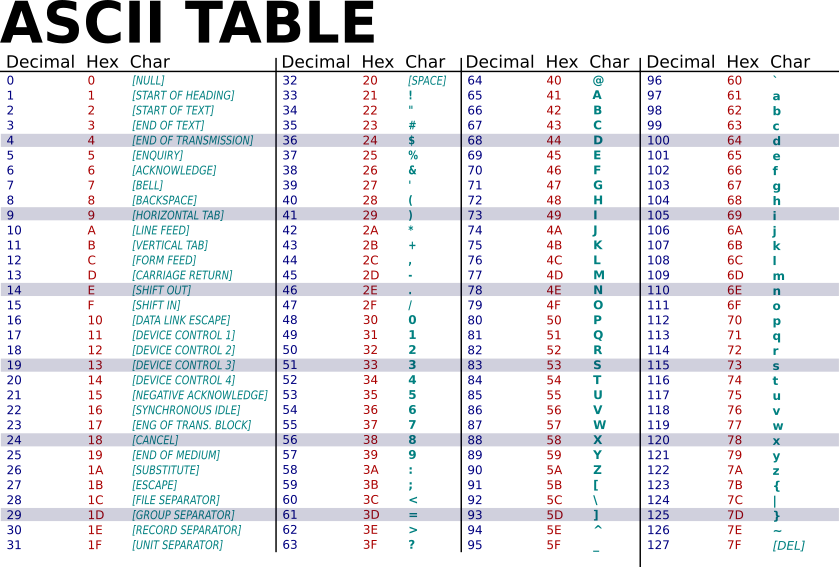
\includegraphics[width=.8\linewidth]{./gfx/ASCII_table}
	\caption[
		ASCII-Tabelle: Lookup-Tabelle zur Interpretation von Zahlen als Schriftzeichen
	]{
		ASCII-Tabelle: Lookup-Tabelle zur Interpretation von Zahlen als Schriftzeichen\\
		Quelle: \url{https://en.wikipedia.org/wiki/File:ASCII-Table-wide.svg}
	}
	\label{fig:ASCII}
\end{center}
\end{figure}

Wenn Sie sich diese Tabelle durchsehen, wird Ihnen auffallen, dass darin auch wieder Ziffern vorkommen. Das bedeutet, dass eine Zahl sowohl durch ihr Bitmuster dargestellt werden kann, als auch durch die Bitmuster ihrer Textdarstellung. Die Zahl \inPy{42} hat etwa das Bitmuster \texttt{00101010}. Als \emph{Text} \inPy{"42"} finden wir dagegen die Schriftzeichen \inPy{"4"} und \inPy{"2"} mit ASCII-Codes 52 und 50 und daher der das Bitmuster \texttt{00110110 00110100}. Genauso kann auch das Bitmuster \texttt{00101010} als das \emph{Schriftzeichen} mit der Nummer 42 gelesen werden, also als \inPy{"*"}.

Bisher mussten wir uns mit der Frage der Interpretation von Daten kaum beschäftigen, da jeder Ausdruck in Python einen zugeordneten \emph{Datentypen} hat; die Regeln zur Interpretation werden also \enquote{kostenlos} mitgeliefert. In Dateien dagegen können wir dagegen nur rohe Daten speichern. Als ProgrammiererInnen müssen wir uns also überlegen, wie und von wem diese Daten interpretiert werden sollen.

Wir unterscheiden im Wesentlichen zwischen \emph{Binärdaten} und \emph{Textdaten}. Binärdaten werden so auf die Festplatte geschrieben, wie sie auch im Speicher vorliegen, und auch so von dort gelesen. Man könnte sagen, Binärdaten seien die Muttersprache der Computer. Textdaten dagegen werden zuerst so übersetzt, dass sie ein menschlicher Leser leicht übersetzen kann.

In einem Beispiel: Sie haben im Speicher die \inPy{int}-Zahl \inPy{42}. Im Binärmodus wird daher das zugehörige Bitmuster \texttt{00101010} auf die Festplatte geschrieben. Öffnen wir diese Datei mit einem \emph{Text}editor, sehen wir das Zeichen \texttt{*}.\\
Wird dieselbe Zahl \inPy{42} dagegen im Textmodus geschrieben, so übersetzt Python diese zuerst in den \emph{Text} \inPy{"42"}, und schreibt dann diesen auf die Festplatte. Wir finden also das Bitmuster \texttt{00110110 00110100}. In einem Texteditor lesen wir auch wieder \texttt{42}.

Python erledigt all dieses Übersetzen für uns im Hintergrund. Wir als ProgrammiererInnen müssen aber zumindest vorgeben, ob eine Datei im Binärmodus oder im Textmodus gelesen/geschrieben werden soll.

\section{Einfacher Dateizugriff}
Python stellt \enquote{einfache Hausmittel} zur Arbeit mit Dateien zur Verfügung. Darauf aufbauend existieren weitere Module, die uns die Arbeit erleichtern, für die wir aber auch die \enquote{Hausmittel} im Prinzip verstanden haben müssen. 

\subsection{Dateien Öffnen und Schließen}
Um mit Dateien umzugehen, brauchen wir zunächst ein \emph{Handle auf die Datei}. Das ist eine Variable, in der alle nötigen Hintergrund-Informationen (Speicherort, Dateigröße, Netzwerkdatei oder lokale Datei, ...) zusammengefasst sind. Es handelt sich also um eine Klasseninstanz, deren Eigenschaften wir hier oberflächlich kennen lernen wollen. Stellen Sie sich das Handle tatsächlich als einen \enquote{Griff} vor, der an eine Datei angebracht wird: mit diesem Griff können Sie die Datei anpacken und darin Operationen (Lesen, Schreiben, Analysieren) durchführen.

Wir erhalten ein solches Handle über den Befehl \inPy{open}:
\begin{codebox}[Syntax: \texttt{open}]
\begin{minted}{python}
handle = open(Dateiname, Modus)
\end{minted}
\end{codebox}

Wie zu erwarten ist \texttt{Dateiname} ein String, der den Namen der Datei enthält, die geöffnet werden soll. Je nach Betriebssystem wird Groß- und Kleinschreibung unterschieden\footnote{Unter Windows wird nicht unterschieden. Linux und Mac dagegen erkennen \texttt{file} und \texttt{File} als unterschiedliche Dateien an.}. Die Datei wird im \emph{aktuellen Arbeitsverzeichnis} erwartet, \ie in dem Ordner, von dem aus Python auch gestartet wurde. Üblicherweise ist das derselbe Pfad, in dem auch Ihre Script-Datei liegt. Sollen Dateien in anderen Ordnern betrachtet werden, können aber auch \emph{absolute} und \emph{relative} Pfadangaben gemacht werden:

Absolute Pfadangaben enthalten die volle Information, wo im Dateisystem eine Datei abgelegt ist. Sie beginnt mit einem Betriebssystem-spezifischen Symbol für die \emph{Wurzel} des Dateisystems (\enquote{root}), und durch \emph{Forward Slashes /}\footnote{Unter Windows sind auch \emph{Backslashes} \textbackslash erlaubt und z.\;T. noch üblich. Dies bereitet aber oft Probleme mit Escape-Sequenzen und sollte daher vermieden werden} voneinander abgetrennte Ordnernamen. Unter Windows ist dieses Wurzel-Zeichen der \emph{Laufwerks-Buchstabe} gefolgt von einem Doppelpunkt. Ein gültiger Dateiname mit absoluter Pfadangabe unter Windows könnte also lauten:
\begin{center}
	\texttt{C:/User/some\_folder/myFile.txt}
\end{center}
Linux und Mac verwalten Laufwerke anders; die Wurzel des Dateisystems ist daher durch einen einfachen Forward Slash gekennzeichnet:
\begin{center}
	\texttt{/home/user/some\_folder/myFile.txt}
\end{center}

Relative Pfadangaben gehen vom aktuellen Arbeitsverzeichnis aus. Von diesem Startpunkt aus wird die Orderstruktur navigiert. Dass eine Pfadangabe relativ sein soll, wird erklärt, indem man als erstes Zeichen einen Punkt angibt.

Beispiel: Ihre Code-Datei liegt unter \texttt{/home/user/Codes/}. Die Datei, die Sie öffnen wollen, befindet sich in \texttt{/home/user/Codes/files}. In dem Fall können Sie auf diese Datei zugreifen, indem Sie als \inPy{Dateiname} angeben:
\begin{center}
	\texttt{./files/myFile.txt}
\end{center}
Dies gilt so gleichermaßen für Windows als auch für Linux und Mac.

Ist die Datei in einem \emph{Überordner}, so kann dies mit \emph{zwei Punkten} angezeigt werden. Wir können auch mehrere ebenen zurück gehen, indem wir Punkte und Slashes aneinander reihen: \texttt{../../} bezeichnet den Ordner \emph{zwei Ebenen} über dem Arbeitsverzeichnis. Weiter können wir diese Schreibweise auch mit relativen Pfadangaben kombinieren. Stellen wir uns wieder vor, das aktuelle Arbeitsverzeichnis wäre \texttt{/home/user/Codes/}. Die Datei, die Sie öffnen wollen, efindet sich nun aber im Order \texttt{/home/user/files}. In diesem Fall geben Sie an:
\begin{center}
	\texttt{../files/myFile.txt}
\end{center}


Unter \emph{Modus} verstehen wir, für welche Art Zugriff die Datei geöffnet werden soll. Wollen wir aus der Datei Lesen oder Schreiben? Soll der Zugriff im Text- oder Binärmodus stattfinden? Der Modus wird durch einen String beschrieben. Die wichtigsten Modi finden Sie in Tabelle \ref{tab:FileModes}:

\begin{center}
\rowcolors{1}{white}{tabhighlight}
\begin{tabular}{c|cp{.6\linewidth}}
	\toprule
	\textbf{String}	& \textbf{Bedeutung}				& \textbf{Kommentar} \tabcrlf
	\texttt{r}				& Lesen -- Textmodus				& Dateicursor am Anfang der Datei.\newline Neuen Dateien werden \emph{nicht} angelegt.\\
	\texttt{rb}			& Lesen -- Binärmodus			& Dateicursor am Anfang der Datei.\newline Neuen Dateien werden \emph{nicht} angelegt.\\
	\texttt{w}				& Schreiben -- Textmodus		& Dateicursor am Anfang der Datei.\newline Neuen Dateien werden angelegt, alte Dateien überschrieben.\\
	\texttt{wb}			& Schreiben -- Binärmodus	& Dateicursor am Anfang der Datei.\newline Neuen Dateien werden angelegt, alte Dateien überschrieben.\\
	\texttt{x}				& Schreiben -- Textmodus		& Dateicursor am Anfang der Datei.\newline Neuen Dateien werden angelegt, alte Dateien \emph{nicht} überschrieben.\\
	\texttt{xb}			& Schreiben -- Binärmodus	& Dateicursor am Anfang der Datei.\newline Neuen Dateien werden angelegt, alte Dateien \emph{nicht} überschrieben.\\
	\texttt{a}				& Anhängen -- Textmodus		& Dateicursor am \emph{Ende} der Datei. Neuen Dateien werden angelegt, alte Dateien \emph{nicht} überschrieben.\\
	\texttt{ab}			& Anhängen -- Binärmodus		& Dateicursor am \emph{Ende} der Datei. Neuen Dateien werden angelegt, alte Dateien \emph{nicht} überschrieben. \\
	\bottomrule
\end{tabular}
\captionof{table}{Dateimodi in Python}
\label{tab:FileModes}
\end{center}

\begin{hintbox}[Relative Pfadangaben bevorzugen]
Absolute Pfadangaben sind von Natur aus unflexibel. Wenn Sie Ihr Programm an Kollegen verschicken, wird es vermutlich nicht mehr funktionieren. Bevorzugen Sie daher relative Pfadangaben, und konzipieren Sie nach Möglichkeit Ihre Programme so, dass notwendige Dateien in \emph{Unterordnern} liegen.
\end{hintbox}

Jede Datei, die geöffnet wurde, sollte auch wieder geschlossen werden. Dies geschieht mit der Methode \inPy{close}:
\begin{codebox}[Syntax: \texttt{open}]
\begin{minted}{python}
handle.close()
\end{minted}
\end{codebox}

Ob eine Datei noch geöffnet ist, können wir mit dem Attribut \inPy{closed} in Erfahrung bringen: \inPy{handle.closed} ist entweder \inPy{True} oder \inPy{False}.

\subsection{Dateien Schreiben}
\subsubsection{Textmodus}
Sobald eine Datei in einem Text-Schreibmodus geöffnet wurde (\texttt{w},  \texttt{x} oder \texttt{a}), und solange sie noch nicht wieder geschlossen wurde, können wir mit der Methode \inPy{write} Text in eine Datei schreiben. Die Syntax ist denkbar einfach:

\begin{codebox}[Syntax: \texttt{write}]
\begin{minted}{python}
handle.write(Text)
\end{minted}
\end{codebox}

Dabei ist \inPy{Text} ein beliebiger Ausdruck, der zu einem String ausgewertet werden kann.

\begin{codebox}[Beispiel: Text-Dateien Schreiben]
\begin{minted}[linenos]{python}
handle = open("output.txt", "w")    # Text/Schreibmodus

handle.write("Some text\n")
handle.write("another line " * 2 + "\n")
handle.write( str(handle) )

handle.close()
\end{minted}
\end{codebox}

\begin{cmdbox}[Dateinhalt von \texttt{output.txt}]
\begin{minted}{text}
Some text
another line another line 
<_io.TextIOWrapper name='output.txt' mode='w' encoding='UTF-8'>
\end{minted}
\end{cmdbox}

Beachten Sie, dass, anders als bei \inPy{print} Zeilenumbrüche \emph{nicht} automatisch angehängt werden. Diese müssen explizit als \inPy{"\n"} teil des zu schreibenden Strings sein.

Im obigen Beispiel wird der \emph{Rückgabewert} der Methode ignoriert. \inPy{write} gibt die Zahl der in die Datei geschriebenen Bytes zurück. Dieses Feature wird selten gebraucht, kann aber unter Umständen nützlich sein.

Öffnen wir nach Zeile dieselbe Datei \texttt{output.txt} nochmals in den Modi \texttt{w}, \texttt{wb}, \texttt{x} oder \texttt{xb}, so wird der Dateiinhalt sofort gelöscht. Bei den Modi \texttt{a} und \texttt{ab} dagegen bleibt der alte Inhalt bestehen; neu geschriebener Text wird an das Ende der Datei angehängt.

\subsubsection{Binärmodus}
Schreiben im Binärmodus funktioniert prinzipiell genauso, wie wir es vom Textmodus schon kennen: Öffnen mit \inPy{open} in einem geeigneten Modus (\texttt{wb},  \texttt{xb} oder \texttt{ab}), Schreiben mit \inPy{handle.write(data)} und Schließen mit \inPy{handle.close()}. An das Objekt \inPy{data} muss \emph{eindeutig} in eine Byte-Sequenz übersetzt werden können. (Eingangs wurde gesagt, dass \eg der \inPy{int}-Wert \inPy{42} in das Bitpattern \texttt{00101010} übersetzt wird; gleichermaßen ist aber auch das Bitpattern \texttt{00000000 00101010} denkbar, und eine beliebige andere Zahl führender Nullen. Die Gründe hierfür sind leider etwas technisch, und können an dieser Stelle nicht erschöpfend erklärt werden).

Eine Klasse von Objekten, das eine solche absolut unmissverständliche Darstellung haben, sind Instanzen der Klasse \inPy{bytes}. Diese können beispielsweise aus \inPy{list}s erstellt werden, wenn deren einzelne Elemente nur Werte zwischen \inPy{0} und \inPy{255} annehmen.

\begin{codebox}[Beispiel: Binär-Dateien Schreiben]
\begin{minted}[linenos]{python}
handle = open("output.dat", "wb")    # Binär/Schreibmodus

data = bytes([65, 66, 67])
handle.write( data )

handle.close()
\end{minted}
\end{codebox}

\begin{cmdbox}[Dateinhalt von \texttt{output.dat}]
\begin{minted}{text}
ABC
\end{minted}
\end{cmdbox}


\subsection{Dateien Lesen}
Das Lesen aus Dateien gestaltet sich ähnlich einfach wie das Schreiben: nachdem die Datei in einem geeigneten Modus geöffnet wurde (\texttt{r} oder \texttt{rb}) kann mit den Methoden \inPy{read} und \inPy{readline} gearbeitet werden.

Beim Lesen können wir uns vorstellen, dass in der Datei ein \enquote{Cursor} platziert wird. Zu Beginn ist dieser ganz am Anfang der Datei. Mit jedem Lese-Befehl wandert dieser Cursor dann vorwärts. Gelesen wird immer jeweils von der aktuellen Cursorposition.

Die Methode \inPy{read} im einfachsten Fall \emph{die gesamte Datei} in den Arbeitsspeicher:
\begin{codebox}[Syntax: \texttt{read}]
\begin{minted}{python}
StringVariable = handle.read()
\end{minted}
\end{codebox}

Optional kann auch ein \inPy{int}-Parameter \inPy{size} mit übergeben werden. Dieser gibt eine Maximalmenge an Daten an, die aus der geöffneten Datei \inPy{handle} gelesen werden dürfen. 
\begin{codebox}[Syntax: \texttt{read} (erweitert)]
\begin{minted}{python}
StringVariable = handle.read(size)
\end{minted}
\end{codebox}
Dabei bezeichnet \inPy{size} die Zahl der Bytes, die maximal gelesen werden dürfen.

Die online-Dokumentation (\url{https://docs.python.org/3/tutorial/inputoutput.html}) kommentiert hierzu lakonisch:
\begin{center}
	\emph{It’s your problem if the file is twice as large as your machine’s memory.}
\end{center}

Beispiel: Wir wollen die im vorigen Abschnitt vorbereitete Datei \texttt{output.txt} zurück in den Arbeitsspeicher lesen. Dies erreichen wir mit dem folgenden Code:
\begin{codebox}[Beispiel: Text-Dateien Lesen]
\begin{minted}[linenos]{python}
handle = open("output.txt", "r")    # Text/Lesemodus

firstWord = handle.read(4)
rest      = handle.read()

handle.close()

print(firstWord)
print(rest)
\end{minted}
\end{codebox}

\begin{cmdbox}[Ausgabe: Text-Dateien Lesen]
\begin{minted}{text}
Some
 text
another line another line 
<_io.TextIOWrapper name='output.txt' mode='w' encoding='UTF-8'>
\end{minted}
\end{cmdbox}

Der Dateiinhalt wird als String in den Speicher geladen. Soll dieser wieder als Zahl behandelt werden, so muss der String mit den entsprechenden Funktionen (\inPy{int()}, \inPy{float()}, ...) umgewandelt werden.

Wird \enquote{nach dem Ende der Datei} versucht, weiter zu lesen, so ist das Ergebnis einfach ein leerer String.

Textdateien sollen besonders häufig Zeile für Zeile bearbeitet werden. Zu diesem Zweck existiert die Methode \inPy{readline}:
\begin{codebox}[Syntax: \texttt{readline}]
\begin{minted}{python}
StringVariable = handle.readline(size)
\end{minted}
\end{codebox}
\inPy{readline} liest von der aktuellen Cursorposition bis zum nächsten Zeilenumbruch. Wieder begrenzt der Parameter \inPy{size} die Datenmenge, die maximal gelesen wird. Wird dieser ausgelassen oder wird hier ein negativer Wert übergeben, so liest Python \emph{die gesamte Zeile}.

Verwandt mit der Methode \inPy{readline} ist die Methode \inPy{readlines}: Diese liest \emph{die gesamte Datei}, zerlegt sie dabei aber bereits an den Zeilenumbrüchen, und packt die Teilde der Datei in eine \inPy{list}:

\begin{codebox}[Beispiel: \texttt{readlines}]
\begin{minted}[linenos]{python}
handle = open("output.txt", "r")    # Text/Lesemodus

lines = handle.readlines()

handle.close()

for line in lines :
    print(line)
\end{minted}
\end{codebox}

Beachten Sie, dass die Zeilenumbrüche selbst beim Lesen nicht entfernt werden. Entsprechend sehen wir bei diesem Beispiel zusätzliche, leere Zeilen:

\begin{cmdbox}[Ausgabe: \texttt{readlines}]
\begin{minted}{text}
Some text

another line another line 

<_io.TextIOWrapper name='output.txt' mode='w' encoding='UTF-8'>
\end{minted}
\end{cmdbox}


\subsection{Dateien und Blockstrukturen}
hintbox -- with -- enter and exit


for line in handle

byteNum = handle.tell()
handle.seek(byteNum)

list(handle)

listOfLines = handle.readlines()

\section{JSON und pickle}


\section{PIL}
